\section{Podlaga za temelje \texttt{LSFEM}}

Kadar obravnavamo prostorsko dinamiko (npr.\ tok tekočine), lahko fizični prostor modeliramo kot 1, 2 ali 3-mnogoterost. Temelje \texttt{LSFEM} bomo polagali na splošnem primeru $d$-mnogoterosti, za ponazoritev pa na njih sproti gradili konkretni 2D primer.

\begin{wrapfigure}{r}{6cm}
	\vspace{-3mm}
	\centering
	\captionsetup{type=figure}
	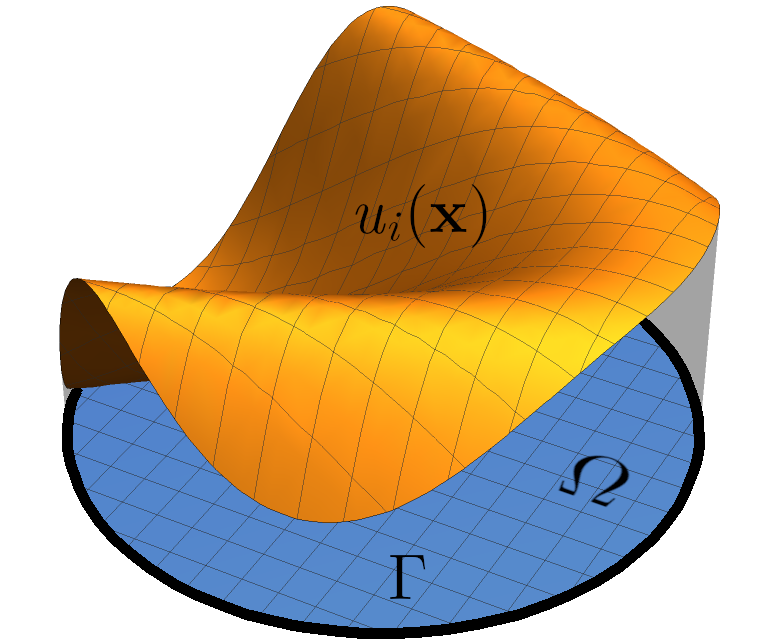
\includegraphics[width=5.5cm]{Slike/funkcijaInDomenaG}
	\caption{Domena $\Omega$, meja domene $\Gamma$ in komponenta rešitve $u_i(\mathbf{x})$.}
\label{fig:funkInDom}
\vspace{0.2cm}
\end{wrapfigure}

Naj bo torej prizorišče dogajanja $d$-mnogoterost $\Omega$ (slika \ref{fig:funkInDom}), opremljena s krajevnim vektorjem:
\vspace{-1.5mm}
\begin{equation}
\mathbf{x} = \{x_1, ..., x_d\} \ . \nonumber
\vspace{-1mm}
\end{equation}
Pri reševanju sistema $m$ \texttt{PDE} iščemo nabor funkcij:
\vspace{-0.5mm}
\begin{equation}
	\mathbf{u}(\mathbf{x}) =  \{u_1(\mathbf{x}), ..., u_m(\mathbf{x})\} \ , \nonumber
	\vspace{-1mm}
\end{equation}
ki v vsaki točki domene $\Omega$ zadosti sistemu \texttt{PDE}, na meji $\Gamma$ pa robnim pogojem. Konkretni primer bomo gradili na 2D primeru s štirimi spremenljivkami, pri katerem bosta krajevni vektor in vektor odvisnih spremenljivk enaka:
\vspace{2.5mm}
\begin{equation}
	\hspace{-60mm} \mathbf{x} = \{x, y\} \quad \text{in} \quad \mathbf{u} =  \{u, v, p, \omega\} \ . \nonumber
\end{equation}
\\[-4mm]
Dinamiko naj opiše \textbf{sistem Stokesovih enačb} za nestisljive tekočine v obliki hitrost-tlak-vrtinčnost, ki jim za večjo nazornost primera umetno dodamo koeficiente $\alpha(\mathbf{x})$, $\beta(\mathbf{x})$, $\gamma(\mathbf{x})$ in $\delta(\mathbf{x})$:\\[0.05cm]
\begin{minipage}{0.11\textwidth}
	\hspace{1cm}
\end{minipage}
\begin{minipage}{0.33\textwidth}
\begin{IEEEeqnarray}{rl}
	\alpha \mkern2mu \frac{\pd p}{\pd x} + \beta \mkern2mu \frac{\pd \omega}{\pd y} & \ = \, f_x \ ,
	\label{eq:StokesXMom}
	\\[0.3cm]
	\gamma \mkern2mu \frac{\pd p}{\pd y} - \delta \mkern2mu \frac{\pd \omega}{\pd x} & \ = \, f_y \ ,
\end{IEEEeqnarray}
\end{minipage}
\begin{minipage}{0.33\textwidth}
\begin{IEEEeqnarray}{rl}
	\frac{\pd u}{\pd x} + \frac{\pd v}{\pd y} & \ = \, 0 \ , \label{eq:StokesDiv}
	\\[0.3cm]
	\omega + \frac{\pd u}{\pd y} - \frac{\pd v}{\pd x} & \ = \, 0 \ .
	\label{eq:StokesCurl}
\end{IEEEeqnarray}
\end{minipage}\\[0.4cm]
Stokesove enačbe ustrezajo stacionarnim Navier-Stokesovim enačbam brez nelinearnih konvektivnih členov, ki jih moramo pri numeričnem reševanju linearizirati. Ker ta korak za ponazoritev \texttt{LSFEM} ni ključen, se mu na tak način izognemo. Stokesove enačbe opisujejo plazeče se tokove, pri katerih je konvekcija gibalne količine (zaradi gibanja) majhna v primerjavi z njeno difuzijo (zaradi viskoznosti).

\setlength{\textheight}{26.4cm}
\pagebreak
\setlength{\topmargin}{1.6cm}			% Header Top Margin Height
\setlength{\headheight}{0.0cm}
\setlength{\headsep}{0.0cm}			% Header Lower Margin Height	 Footer height
\fancyhf{}
\fancyfoot[C]{\thepage}

V enačbah ni časovnih odvisnosti (razen preko časovno odvisnih robnih pogojev), zato so takšni tokovi časovno obrnljivi: časovno obrnjena rešitev enačb je prav tako rešitev (slika \ref{fig:TaylorCouette}).

\begin{figure}[!ht]
	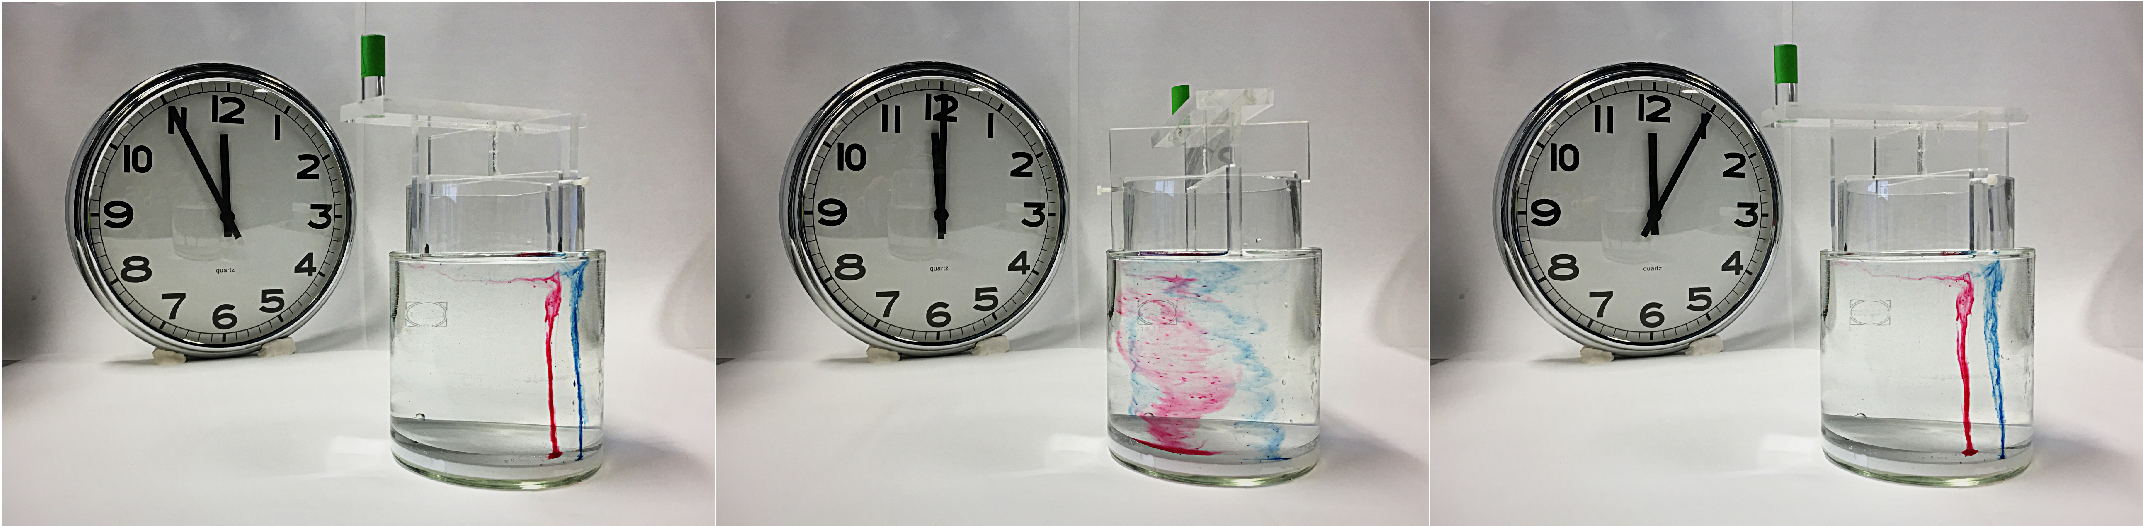
\includegraphics[width = 1\textwidth]{Slike/TaylorCouette}
	\caption{Zabaven eksperiment, pri katerem se v ozkem prostoru med dvema koncentričnima valjema nahaja viskozna tekočina, ki jo na dveh mestih označimo z liso barvila. Valja pet minut vrtimo v nasprotnih smereh (Stokesov tok, ki tako nastane, imenujemo Taylor-Couettov tok), da se lisi pomešata, nato smeri vrtenja obrnemo in po petih minutah se lisi ponovno sestavita. Pridobljeno iz  \cite{Wiki-StokesFlow}.}
	\label{fig:TaylorCouette}
\end{figure}

Sistem \texttt{PDE}, ki ga obravnavamo, zapišemo bolj jedrnato v matrični obliki. To je enostavno, če je sistem linearen. Uvedemo diferencialni operator $\mathbsf{A}$:
\begin{equation}
	\mathbsf{A}(\mathbf{x}) \mkern2mu
	=
	\, \mathbsf{A}_0(\mathbf{x}) + \mathbsf{A}_1(\mathbf{x}) \frac{\pd}{\pd x_1} + \, \mathbsf{A}_2(\mathbf{x}) \frac{\pd}{\pd x_2} \ ,
	\label{eq:AMatrixDefinition}
	\vspace{-1mm}
\end{equation}
\vspace{1mm}
s katerim lahko sistem enačb zapišemo kot:
\begin{equation}
	\left(\mathbsf{A}_0(\mathbf{x}) + \mathbsf{A}_1(\mathbf{x}) \mkern1mu \frac{\pd}{\pd x_1} + \mathbsf{A}_2(\mathbf{x}) \mkern1mu \frac{\pd}{\pd x_2}\right) \mkern-1mu \cdot \mkern-1mu \mathbf{u}(\mathbf{x}) \, = \, \mathbf{f}(\mathbf{x}) \ ,
	\label{eq:matrixPDE1}
	\vspace{-1mm}
\end{equation}
oziroma na kratko:
\vspace{2mm}
\begin{equation}
	\hspace{12mm} \boxed{
		\, \vphantom{\big(} \mathbsf{A}(\mathbf{x}) \mkern-1.5mu \cdot \mkern-1.5mu \mathbf{u}(\mathbf{x}) = \, \mathbf{f}(\mathbf{x}) \,
	}\hspace{1.3cm} \texttt{sistem PDE .}
	\label{eq:compactPDE}
	\vspace{1.5mm}
\end{equation}
V matriko $\mathbsf{A}_0$ spravimo vse koeficiente pred členi z odvisnimi spremenljivkami, v matriko $\mathbsf{A}_1$ vse koeficiente pred členi z odvodi odvisnih spremenljivk po koordinati $x_1$ in v $\mathbsf{A}_2$ vse koeficiente pred členi z odvodi odvisnih spremenljivk koordinati $x_2$. Ostale člene zložimo v vektor $\mathbf{f}$. Enačbe \eqref{eq:StokesXMom} - \eqref{eq:StokesCurl} lahko po zgledu enačbe \eqref{eq:matrixPDE1} zapišemo kot:
\vspace{1.5mm}
\begin{equation}
	\left[ \,
	\begin{pmatrix}
		0 & 0 & 0 & 0 \\
		0 & 0 & 0 & 0 \\
		0 & 0 & 0 & 0 \\
		0 & 0 & 0 & 1
	\end{pmatrix} +
	\begin{pmatrix}
		1 & 0 & 0 & 0 \\
		0 & 0 & \alpha & 0 \\
		0 & 0 & 0 & -\delta \\
		0 & -1 & 0 & 0
	\end{pmatrix} \frac{\pd}{\pd x} +
	\begin{pmatrix}
		0 & 1 & 0 & 0 \\
		0 & 0 & 0 & \gamma \\
		0 & 0 & \beta & 0 \\
		1 & 0 & 0 & 0 \\
	\end{pmatrix} \frac{\pd}{\pd y} \, \right]
	\ \cdot \
	\begin{pmatrix}
		u(\mathbf{x}) \\ v(\mathbf{x}) \\ p(\mathbf{x}) \\ \omega(\mathbf{x})
	\end{pmatrix}
	\ = \
	\begin{pmatrix}
		0 \\ f_x(\mathbf{x}) \\ f_y(\mathbf{x}) \\ 0
	\end{pmatrix} \ .
	\vspace{1mm}
\end{equation}